\section{Requirement engineering process}

Inadequate requirements are widespread, and the process of requirement engineering is both challenging and pivotal. 
This is because issues in the initial stages can potentially escalate costs by a factor of up to two hundred during the final phase.
\begin{figure}[H]
    \centering
    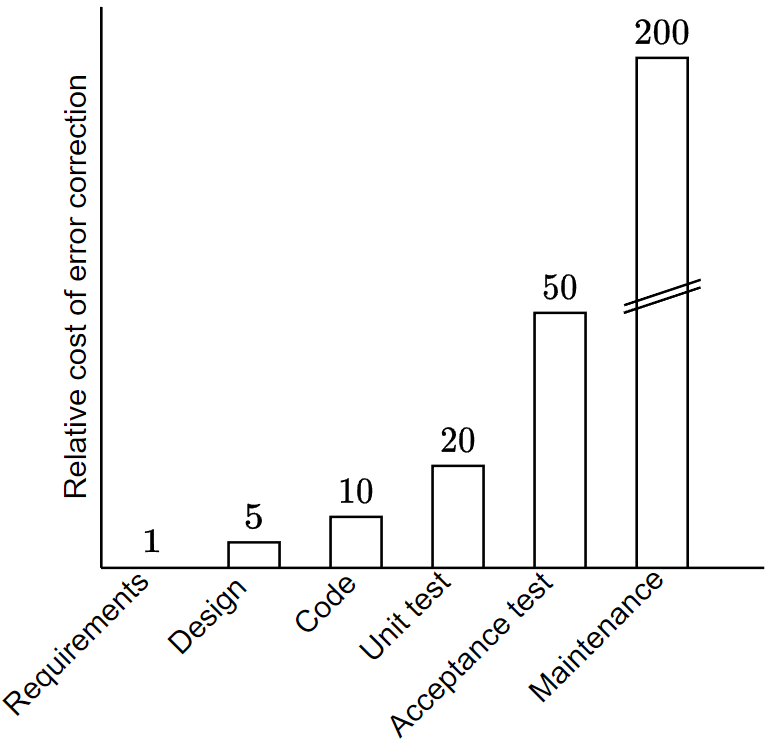
\includegraphics[width=0.35\linewidth]{images/requirements.png}
    \caption{Cost of late correction [Boehm, 1981]}
\end{figure}
The complexity of requirement engineering arises from several factors, including composite systems, the presence of multiple systems, varying abstraction levels, diverse concerns, and involvement of stakeholders with different backgrounds.

Requirement engineers are tasked with various responsibilities, including:
\begin{itemize}
    \item Eliciting information, which involves gathering details about project objectives, context, scope, domain boundaries, and requirements.
    \item Modeling and analysis, encompassing the definition of goals, objects, use cases, and scenarios.
    \item Communicating requirements, which includes providing analysis feedback, documenting in the Requirements Analysis and Specification Document (RASD), and creating system prototypes.
    \item Negotiating and agreeing upon requirements, which involves resolving conflicts and managing risks, assisting in requirement selection and prioritization.
    \item Managing and evolving requirements, involves overseeing them across the entire development lifecycle, ensuring backward and forward traceability, and effectively managing changes and their consequences.
\end{itemize}